\documentclass[tikz,border=8pt]{standalone}
\usepackage{amsmath}
\begin{document}
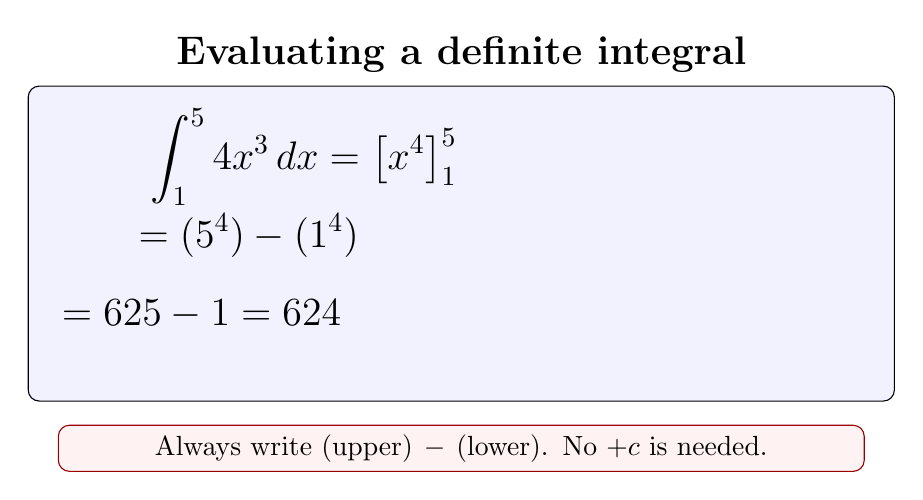
\begin{tikzpicture}
\node[font=\Large\bfseries] at (0,3) {Evaluating a definite integral};
\node[draw,rounded corners,fill=blue!5,minimum width=11cm,minimum height=4cm] at (0,0.6) {};
\node[font=\Large] at (-2,1.7) {$\displaystyle \int_1^5 4x^3\,dx=\left[x^4\right]_1^5$};
\node[font=\Large] at (-2.7,0.7) {$\displaystyle =(5^4)-(1^4)$};
\node[font=\Large] at (-3.3,-0.3) {$\displaystyle =625-1=624$};
\node[draw=red!60!black,rounded corners,fill=red!5,align=center,text width=10cm] at (0,-2)
{Always write \((\text{upper})-(\text{lower})\). No \(+c\) is needed.};
\end{tikzpicture}
\end{document}